%!TEX root = main.tex

% Introduction for negFE
\section{Introduction}
Infromation reconciliation and privacy amplification are the two fundamental tasks for key derivation from noisy sources used in quantum key agreement, biometrics, and physically uncloneable functions. Secure sketches perform information reconciliation non-interactively.  Specifically, they consist of a pair of algorithms $\sketch$ where $\sketch(w) = \sketch$ should reveal as little information as possible about $w$.  Simultaneously it should be the case that for all nearby $w', \rep(w', \sketch) = w$.  The tension is that, $\sketch$ has to have enough information about $w$ to reconstruct it from any nearby value.  Fuzzy extractors additionally convert $w$ into a uniform value.  They consist of a pair $(\gen, \rep$) where $(r, p)\leftarrow \gen(w)$ is indistinguishable from $(u, p)$ and $\rep(w', p) =r$.

Throughout the introduction we use the notation of fuzzy extractors, the discussion also applies to secure sketches. 
Since noisy sources come from the physical world the goal is to be able to support as many distributions $W$ as possible.  Fuller, Reyzin, and Smith~\cite{fuller2016fuzzy,fuller2020fuzzy} identified the notion of fuzzy min-entropy $\Hfuzz(W)$ which measures the adversary's success when given oracle access to $\rec(\cdot, p)$ but is unable to learn anything from the values  $p$.  Mathematically,
\[
\Hfuzz(W):= -\log{\max_{w'} \sum_{w | \dis(w, w')\le t} \Pr[W=w]}.
\]A primary goal of fuzzy extractors is to build a single fuzzy extractor that works for the family of all distributions $\Wallfuzz = \{ W | \Hfuzz(W) = \omega(\log \lambda)$ for some security parameter $\lambda$.  If one desires computational security, this is achievable using general obfuscation~\cite{BitanskyCKP14,bitansky2017virtual} or specific number-theoretic assumptions~\cite{galbraith2019obfuscated}. 

Fuzzy extractors have long been considered an information-theoretic primitive given the strong connections to randomness extraction and coding theory.  Unfortunately, the situation for information-theoretic security is more complicated.  Fuller, Reyzin, and Smith~\cite{fuller2020fuzzy} showed that it is impossible to build a fuzzy extractor for the family $\Wallfuzz$.  On the positive side, multiple works~\cite{hayashi2014secret,hayashi2016secret,fuller2016fuzzy,woodage2017new,tyagi2017universal,TVW18,LA18,fuller2019continuous,fuller2020fuzzy} presented a construction that works for each $W\in \Wallfuzz$.  This is called the \emph{distribution-sensitive} setting as one knows the entire probability mass function of the chosen $W$, denoted as $\gen_W, \rec_W$.  All constructions in this line are computationally inefficient; for an input point $w$ they look up the probability that $\Pr[W=w]$, so they crucially rely on storing this probability mass function.  
The primary question of this work is:
\begin{displayquote}
Are there efficient information-theoretic fuzzy extractors in the \emph{distribution-sensitive} setting? 
\end{displayquote}

We answer the above negatively.  Consider the Hamming metric over $\zo^n$. For most distributions $W$ where $\Hfuzz(W) := \gamma$ building a good fuzzy extractor requires having approximately $\gamma 2^\gamma$ bits of information about the distribution. The actual distributions we consider have more points than their fuzzy min-entropy.  These constructions have $2^k$ points where $k = \gamma + c n$ for an arbitrary constant $c>0$, impossibility is when storage is $o(k2^k)$.  In spirit, our impossibility result rules out constructions that do not have a full description of the probability mass function written in their description.  The relevant parameter regimes of impossibility are shown in Figure~\ref{fig:param regime} with the area under the curves representing parameters where the construction is impossible for an average distribution unless one has $\Theta(k 2^k)$ bits of information about the distribution.  


\begin{figure*}[t]
\centering
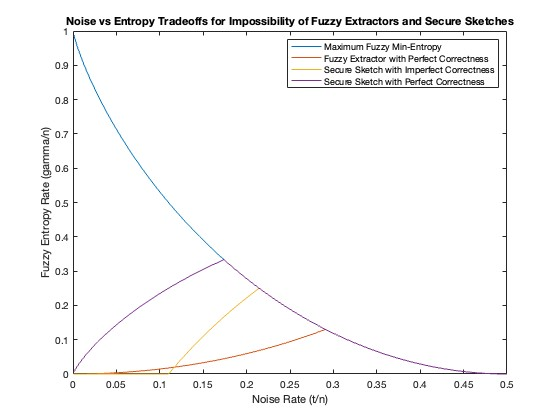
\includegraphics[width=.8\textwidth]{EntropyvsError.jpg}
\caption{The region of error rate $t/n$ ($x$-axis) and fuzzy entropy rate $\gamma/n$ (y-axis) pairs for which the two negative results apply.  The four curves are maximum fuzzy min-entropy, Theorem~\ref{thm:main theorem}, Theorem~\ref{thm:main theorem ss} with $\delta=.25$, and Theorem~\ref{thm:main theorem ss} with $\delta =0$.}
\label{fig:param regime}
\end{figure*}

There are two natural interpretations of the above result: 1) that fuzzy min-entropy does not measure the suitability of distributions for key derivation or 2) that fuzzy extractors are an inherently computational object.

\paragraph{The notion of fuzzy min-entropy}
Talk about how traditional randomness extraction~\cite{nisan1993randomness} $\Hoo(W)$ represents exactly the strength of guessing the key with having oracle access to the primitive. What could you do to avoid the result?

\paragraph{Fuzzy extractors are computational}

\subsection{Proof Techniques}
The core of our negative results show impossibility of a fuzzy extractor variant that directly encodes the information available to $(\gen, \rep)$ about the distribution $W$.  Specifically, we know consider a tuple of algorithms $(\advise, \gen, \rep)$ and the following game:
\begin{enumerate}
\itemsep0em
\item A uniform sample from $W_z\leftarrow \mathcal{W}$ where $z$ describes the distribution.
\item A bounded length $\advise = \advise(z)$ is computed.
\item One computes $w\leftarrow W_z$.
\item The algorithm computes $(r, p)\leftarrow \gen(w, \advise)$.
\item The adversary is given either $(r, p, z)$ or $(u, p, z)$ for a uniform $u$.
\end{enumerate}
We call this a \emph{fuzzy extractor with distributional advise}.  Hardness of building such a primitive for an average $z$ implies that an average $z$ does not have a description with less than $|\advise|$ bits~\ref{lem:distributional advise suffices}. 

We consider the set of distributions $\{W_Z\}$ of all distributions with fuzzy min-entropy $\gamma$.  This distribution is statistically close to the set of all distributions with $2^k$ points chosen uniformly without replacement where $k = \gamma +cn$ for an arbitrary constant $c>0$.  We call this set of distributions $U_{n,k}$ and let $w_1,...., w_{2^k}$.  Since the  $2^k$ points are minimally correlated, as long as $|\advise|$ is shorter than $k2^k$, most points $w_i | \advise$ are unpredictable.  

Once one has a bound on the predictability of points in $w_i$, one can use the correctness guarantees of the fuzzy extractor to show that:
\begin{enumerate}
\item Not all points $w\in\zo^n$ are viable for a particular value of $p$.  For a realistic $w$ all nearby points should map to the same key.
\item Since the values of $w_i$ are unpredictable given $\advise$ very few of the $w_i$ will be included in the set of viable points.
\item The adversary knowing $z$ can check the intersection between $w_i$ and $\viable$ points.  
\item If the expected size of the intersection is smaller than the number of keys, then for some keys there is no explanation in terms of a viable $w_i$.
\item Keys with no viable explanation must belong to the uniform distribution.
\end{enumerate}

The techniques for the secure sketch setting are similar, however, there are stronger geometric bounds on the number of viable points since secure sketches imply Shannon error correcting codes.  Crucially, our result considers a secure sketch that retains smooth min-entropy instead of min-entropy.  This is so we can use $U_{n,k}$ throughout the proof and show this implies the hardness of building a secure sketch for all distributions with sufficient fuzzy min-entropy.  


Importantly, both results operate generically in the size of the maximum number of viable points for the relevant primitive.  Such bounds have been well established in the literature due to their connections with coding theory.  This means if one can provide a new bound on fuzzy extractor or secure sketch quality this can be directly used in our results.
